\documentclass[a4paper,9pt]{extarticle}

%=========================================================
% PACKAGES
%=========================================================

\usepackage[
a4paper,
top=1.8cm,
bottom=1.5cm,
footskip=7mm,
left=1cm,
right=1cm,
headheight=14pt,
headsep=5mm
]{geometry}
\usepackage[T1]{fontenc}
\usepackage[utf8]{inputenc}
\usepackage[french]{babel}

\usepackage[sfdefault]{FiraSans}
\renewcommand{\familydefault}{\sfdefault}

\usepackage{multicol}
\setlength{\columnsep}{0.7cm}

\usepackage{amsmath,amssymb}

\usepackage{titlesec}
\usepackage{enumitem}

\usepackage{tcolorbox}
\tcbuselibrary{skins,breakable}

\usepackage{xcolor}

\usepackage{graphicx}
\usepackage{float}

\usepackage{tikz}

\usepackage{fancyhdr}
\usepackage[hidelinks]{hyperref}


%=========================================================
% PAGE SETTINGS
%=========================================================

\setlength{\parindent}{0pt}
\setlength{\parskip}{1.5pt}

\setlength{\abovedisplayskip}{4pt}
\setlength{\belowdisplayskip}{4pt}

\setlist[itemize]{
leftmargin=*,
itemsep=1pt,
topsep=1pt
}


%=========================================================
% COLORS
%=========================================================

\definecolor{Blue}{HTML}{E3F0FF}
\definecolor{Green}{HTML}{E3F7EA}
\definecolor{Pink}{HTML}{FFE5ED}
\definecolor{Orange}{HTML}{FFF0DC}
\definecolor{Purple}{HTML}{EEE7FF}
\definecolor{Yellow}{HTML}{FFFADB}


\definecolor{BlueTitle}{HTML}{285B8F}
\definecolor{GreenTitle}{HTML}{287052}
\definecolor{PinkTitle}{HTML}{A84063}
\definecolor{OrangeTitle}{HTML}{A96500}
\definecolor{PurpleTitle}{HTML}{6245A5}


%=========================================================
% HEADER
%=========================================================

\pagestyle{fancy}

\fancyhf{}

\fancyhead[L]{\small\textbf{Game Theory and Strategic Decisions}}
\fancyhead[C]{\small Backward Induction Paradoxes and Bayesian Games}
\fancyhead[R]{\small Week 04 --- 28/09-04/10/2026}

\fancyfoot[C]{\small\href{https://github.com/AlphaXT38G/notes_ba5}{github.com/AlphaXT38G/notes\_ba5}}
\fancyfoot[R]{\small \thepage}

\renewcommand{\headrulewidth}{0.4pt}



%=========================================================
% TITLES
%=========================================================

\titleformat{\section}
{\large\bfseries\color{BlueTitle}}
{}{0pt}{}

\titlespacing{\section}
{0pt}{6pt}{3pt}


% separator

\newcommand{\separator}{
\vspace{2pt}
\hrule
\vspace{3pt}
}


%=========================================================
% BOXES
%=========================================================

% Boxes are kept whole (unbreakable): inside multicols, a box split by tcolorbox
% leaves an empty column behind it.

% DEFINITION - blue
\newtcolorbox{definition}{
enhanced,
unbreakable,
colback=Blue,
colframe=BlueTitle,
boxrule=0.7pt,
arc=0mm,
title=\textbf{Definition},
fonttitle=\bfseries
}

% IMPORTANT - pink
\newtcolorbox{important}{
enhanced,
unbreakable,
colback=Pink,
colframe=PinkTitle,
boxrule=0.7pt,
arc=0mm,
title=\textbf{Key idea},
fonttitle=\bfseries
}

% FORMULAS - green
\newtcolorbox{formula}{
enhanced,
unbreakable,
colback=Green,
colframe=GreenTitle,
boxrule=0.7pt,
arc=0mm,
title=\textbf{Key formulas},
fonttitle=\bfseries
}

% WARNING - orange
\newtcolorbox{warning}{
enhanced,
unbreakable,
colback=Orange,
colframe=OrangeTitle,
boxrule=0.7pt,
arc=0mm,
title=\textbf{Warning},
fonttitle=\bfseries
}

% EXAMPLE - purple
\newtcolorbox{example}{
enhanced,
unbreakable,
colback=Purple,
colframe=PurpleTitle,
boxrule=0.7pt,
arc=0mm,
title=\textbf{Example},
fonttitle=\bfseries
}

% SUMMARY - orange
\newtcolorbox{summary}{
enhanced,
unbreakable,
colback=Yellow,
colframe=OrangeTitle,
boxrule=0.7pt,
arc=0mm,
title=\textbf{Summary},
fonttitle=\bfseries
}



%=========================================================
% FIGURE BOX
%=========================================================

\newtcolorbox{figurebox}{
enhanced,
colback=white,
colframe=gray,
boxrule=0.5pt,
arc=0mm,
center
}



%=========================================================
% DOCUMENT
%=========================================================

\begin{document}

%\footnotesize   --> To reduce the size of the text

\thispagestyle{fancy}



\begin{multicols}{2}



%=========================================================
\section{This Week's Plan}


\begin{important}

\begin{itemize}

\item Last week: the Nash equilibrium is unsatisfactory for sequential games; we introduced
\textbf{Subgame-perfect equilibria}, found by \textbf{backward induction}.

\item This week: more sequential games, with a common theme: \textbf{backward induction can
also lead to unrealistic and unintuitive solutions}.

\item New topic: games of incomplete information, also called \textbf{Bayesian games}.

\end{itemize}

\end{important}



%=========================================================
\section{The Pirate Game}


\begin{example}

\textbf{Rules} -- 5 pirates A, B, C, D, E share 100 coins.

\begin{itemize}

\item Captain A proposes how to split the 100 coins. If at least \textbf{half} (3 in this
case, including himself) the pirates vote yes, the vote passes.

\item If the vote does not pass, A is killed and B becomes captain, and makes a new proposal,
that needs to be voted by at least half (2 in this case) of the remaining pirates, otherwise B
is killed and C becomes captain\dots

\item A pirate needs to be \textbf{strictly better off} with the proposed plan than in the
continuation of the game to vote yes.

\end{itemize}

What's the Subgame-Perfect equilibrium? Will captain Amaro be thrown in the ocean? If not,
how many of the 100 coins will he be able to keep?

\end{example}


\textbf{Pirates left at each time}

\begin{center}
\begin{tabular}{ccccc}
t=1 & t=2 & t=3 & t=4 & t=5 \\
\hline
A & B & C & D & E \\
B & C & D & E & \\
C & D & E & & \\
D & E & & & \\
E & & & & \\
\end{tabular}
\end{center}


\begin{formula}

\textbf{Backward induction} (coins of A, B, C, D, E; ``--'' = already killed)

\begin{itemize}

\item \textbf{t=4} (D, E): D's own vote is half of 2: D keeps everything.
\hfill (--, --, --, 100, 0)

\item \textbf{t=3} (C, D, E): C needs 2 votes. E gets 0 at t=4, so 1 coin makes him strictly
better off. \hfill (--, --, 99, 0, 1)

\item \textbf{t=2} (B, C, D, E): B needs 2 votes. D gets 0 at t=3: 1 coin buys his vote.
\hfill (--, 99, 0, 1, 0)

\item \textbf{t=1} (A, \dots, E): A needs 3 votes. C and E get 0 at t=2: 1 coin each.
\hfill (98, 0, 1, 0, 1)

\end{itemize}

\end{formula}


\begin{important}

\textbf{SPE}: captain A proposes $(98, 0, 1, 0, 1)$; A, C and E vote yes. He is not thrown
in the ocean, and keeps \textbf{98 coins}.

\end{important}



%=========================================================
\section{The Centipede Game}


\begin{center}

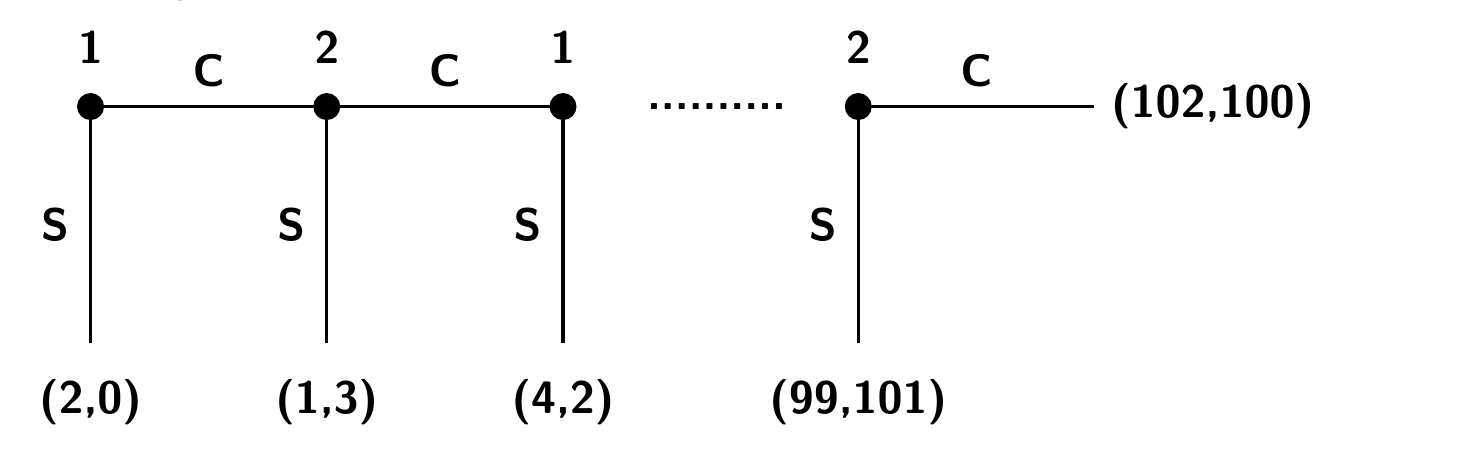
\includegraphics[
width=\linewidth
]{../images/week04_01.png}

\end{center}


\begin{example}

\begin{itemize}

\item Players: 1 and 2, moving in turn: Continue (C) or Stop (S).

\item In each period, the total payout (sum of the payouts of Player 1 and Player 2)
increases by 2 units. One would think players would want to continue playing as long as
possible.

\end{itemize}

\end{example}


\begin{important}

\textbf{Backward induction}

\begin{itemize}

\item At the last node, it's optimal for Player 2 to stop: (99,101) instead of (102,100).

\item At each node, knowing that at the next node the other player will stop, the player who
moves at that time finds it optimal to stop.

\item The unique SPE involves Player 1 stopping at the first node, with payout
\textbf{(2,0)}: each player quits at every node.

\end{itemize}

Lost opportunity to gain a total of up to 202 for the players! Is backward induction
realistic?

\end{important}


\begin{example}

\textbf{The Centipede game in the lab}

\begin{itemize}

\item People asked to play this game typically do not quit in the first stages.

\item Interpretation: people have a higher tendency to collaborate than predicted by the
model. They understand that if they both continue, their payout will increase over time, so
they take the risk to continue, which pays off if also the other player continues.

\item Different from the Prisoner Dilemma: one player has an incentive to cooperate if also
the other player cooperates.

\end{itemize}

\end{example}



\end{multicols}


\end{document}
